\chapter{Introduction} \label{ch:introduction}

\section{Background}
Approximately 18 million patients are diagnosed with cancer each year
\cite{Bray2019}, with reports indicating that up to 50\% of all cases could
benefit from radiotherapy (RT) for curative or palliative management of disease
(optimal radiotherapy utilisation rate) \cite{Barton2014}. Treatment planning
for RT involves the optimisation of beam quality, field arrangements, dose
distributions, and fractionation schedules, to both maximise tumour
control probability and minimise normal tissue complication probability - 
maximising the therapeutic ratio of treatment \cite{iaea2016}. Contouring (or
delineation) is a critical aspect of treatment planning that describes the
process of defining and classifying anatomical regions-of-interest (ROIs) within
a patient from medical imaging data \cite{iaea2016}. Regions include: target
volumes for treatment, associated error margins; as well as normal tissue
regions (organs at risk - OARs) for which exposure needs to be minimised to
avoid adverse side-effects of treatment \cite{iaea2016}. Once ROIs are
delineated, they are used within the treatment planning system for the
calculation of an optimum dose distribution (as seen in Figure
\ref{fig:contour}). Therefore, contours are part of the primary geometry used to
optimise treatment outcomes; and as such, accurate contouring is fundamental to
the efficacy of RT \cite{Nikolov_2018}.

\begin{figure}[h]
	\begin{center}
		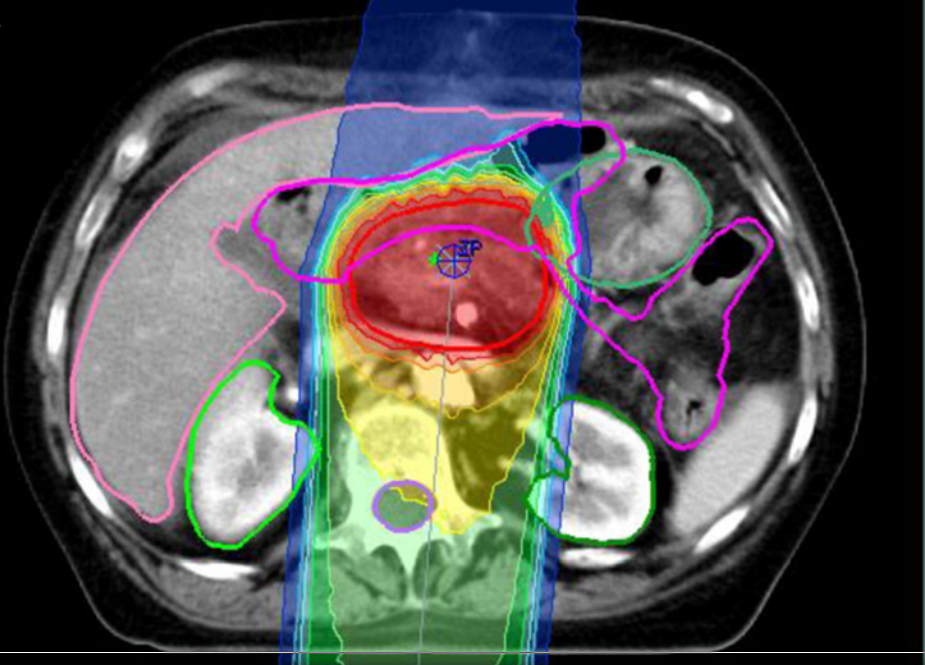
\includegraphics[width=0.5\textwidth]{contour}
		\caption{Single posterior field setup for carbon ion radiotherapy treatment
      of pancreatic cancer. Multiple contours are outlined on diagnostic CT
      imaging for treatment planning. Colour map shows the dose distribution
      over patient anatomy. Figure redrawn from Dreher et al. \cite{Dreher2017}.}
		\label{fig:contour}
	\end{center}
\end{figure}

However, there are current limitations to contouring in clinical practice. Large
intra- and inter-practitioner (observer) variability (IOV) exists in the
definition of ROIs generated from medical imaging. IOV is a long-standing
challenge in RT, and is frequently reported as the largest source of error in
accurate treatment delivery \cite{Vinod_2016, tg100}. Additionally, manual
contouring is both time consuming and requires skilled experts
\cite{Nikolov_2018}. For instance, research has estimated that a radiation
oncologist (RO) needs between 90 -- 120 minutes to delineate pelvic OARs in a
cervical cancer patient \cite{Liu_2020}. In practice, the process is often
computer aided with automatic OAR segmentation tools (i.e. deformable image
registration or atlas-based methods) which has reduced contouring times and
improved consistency between expert observers \cite{Vinod_2016}. However,
atlas-based methods still require significant manual correction 
\cite{Nikolov_2018}, and experience difficulty with small organ volumes, regions
with poor contrast for border differentiation, or high variability in size or location
- such as pelvic OARs in prostate and cervical cancer \cite{Schreier_2020,
Liu_2020}. Critically, current automatic solutions still present a barrier to
the adoption of future technologies that would require fast and accurate
contouring \cite{Nikolov_2018}. For instance, adaptive radiotherapy has shown
potential to deliver a new standard of care for RT patients by updating
treatment plans to daily changes in patient anatomy \cite{Nikolov_2018}.

In contrast, deep-learning (DL) algorithms have shown significant performance
improvements over atlas methods both in terms of accuracy and time for contour
generation \cite{Liu_2020}. However, the implementation of DL models in clinical
environments remains challenging; particularly due to limitations in
quantitatively assessing model performance in comparison to expert performance
and IOV \cite{Nikolov_2018}. Typical metrics used to quantify the similarity
between model and expert contours are volumetric in nature, hence volume overlap
tends to be the focus of evaluation and model optimisation \cite{Nikolov_2018}.
Recent studies have introduced surface-based performance metrics that aim to
provide direct information on the fraction of surface points that require
correction to be within IOV tolerances (specific to each OAR)
\cite{Nikolov_2018, Vaassen_2020}, and may provide a stronger correlation with
time required for contour correction \cite{Vaassen_2020}.

U-Net is a type of deep-learning architecture that leverages multi-resolution
analysis to perform state-of-the-art segmentation in medical imaging research
\cite{Kazemifar_2018, Zhu_2018}. This study presents two independent U-Net
models in an attempt to address a perennial automation problem in the field of
RT.

\section{Aim}


\textbf{Model 1 - Pelvic imaging QA tool}

Model 1 was designed to fulfil the need for IOV comparisons to become part of
regular quality assurance for contour generation \cite{Vinod_2016}; and, to
evaluate the ability of a U-Net architecture to achieve expert level performance
- as defined by Nikolov et al.'s surface dice similarity coefficient (sDSC)
\cite{Nikolov_2018}. This study focused on pelvic CT, automatically
contouring the patient, bladder and rectum volumes. These organs were selected
for their relative ease of contouring when compared to other structures (i.e. head
and neck) \cite{Wong2020}, with the intent to act as a template for future work
extending to other organs.

\textbf{Model 2 - Automatic segmentation of vacuum bag structures in canine
imaging}

Model 2 was designed to automatically contour the vacuum bag structure used to
position and stabilise patients for canine CT and RT. Vacuum bag structures are
reported to take approximately 30 minutes per patient to contour; and hence,
this model aims to automate a time-consuming aspect of RT treatment that is
currently processed manually at SASH veterinary clinic.


